\chapter{Evaluation}
\label{chap:Evaluation}

The goal of this chapter is to evaluate different use-cases for ML-based interpolation in the context of air temperature interpolation. In Chapter~\ref{chap:Machine Learning based Interpolation}, different models for ML-based interpolation were already introduced. Afterwards, the available data and features were introduced in Chapter~\ref{chap:preparations data sets}. In this chapter, the different models are compared with different datasets and features to test the feasibility of two main use cases:

\begin{enumerate}
  \item Interpolation of air temperature for a specific location
  \item Areal interpolation of air temperature
\end{enumerate}

Next to these main uses cases we discuss in this work, the different regression models can be used in many other ways, primarily based on the features used during training. Some regression models could for example be used to predict future air temperature as well, however this is out of the scope of this work.

\subsubsection{Implementation Details}

All ML models are implemented using Python and the scikit-learn library~\cite{scikit-learn}. Additionally the following libraries are used:

\begin{itemize}
  \item Pandas, Numpy, Geopandas, scipy, matplotlib, shapely, contextily, pytz, sklearn, seaborn, rasterio, polars, Google Earth Engine, pykrige, pytorch, missingno
\end{itemize}

\subsubsection{Validation Methodology}
\label{sec:validation methodology}

In order to validate the different models, we use the following methodology:\\
\\
We evaluate two locations based on data availability, e.g. Hamburg and Stuttgart, that also have slightly different climate characteristics, tho both are located in Germany in a moderate cool climatic zone, with Hamburg located near the coast in rather maritim climate and Stuttgart located more inland in a continental climate. Hamburg has also higher precipitation and wind compared to Stuttgart.
For both locations, we collected PWS data from Netatmo and Sensor.Community, however Netatmo data is only available for the whole month of June 2023 for Hamburg and for a single timestep on 19. June 2023 14h for Stuttgart, while Sensor.Community data is available for the whole months of January and June 2023 for both locations.\\
For both locations for both interpolation use-cases, we first compare all available models, e.g. Linear Regression (baseline), KNN, Random Forest, SVM, and Histogram-based Gradient Boosting, with all features against each other to get an understanding of the overall performance of the models and maximum achivable potential, given the assumption that more features generally improve prediction quality. The datasets are split into a training and test set. 70\% of the data is used for training and 30\% is completely withhold for testing. The training and test set are split randomly. The same split is used for all models and sensors to ensure comparability.
Afterwards, the most promising model with the lowest error is used to further evaluate specific influences such as distances between neighbours or the amount of training data and time intervals. For the further evaluation, 5-Fold Cross Validation is used in order to reduce the risk of overfitting~\cite{kohavi1995study}. We note here, that a k of 10 would be preferred, however due to the computational overhead we only use a k of 5 for exploration.\\
All ML models in the initial evaluation are trained using the default parameters as defined in the scikit-learn library. The only exception is the number of estimators for the Random Forest Regressor and the number of iterations for the Histogram-based Gradient Boosting Regressor, which are both increased from 100 to 200 to improve the performance of the models as found out by previous exploration. In order to get the best possible performance of each model, an exhaustive grid search would be prefered for all models in order to fine-tune all hyperparameters, however due to the computational overhead of running exhaustive grid searches, this is not feasible in the scope of this work.\\
For the error metrics, the following candidates are available: MSE, MAE, RSME, R2. MSE is the most commonly used error metric and is more sensitive to outliers, whereas MAE punishes outliers less but is therefore also more variable. Related work commonly uses RSME as it has the same unit as the response variable, therefore RSME is used as the main error metric. R2 is additonally used to get an understanding of the variance of the model.

\section{Interpolation of Air Temperature for a Specific Location}

The first use-case to be evaluated is the interpolation of air temperature for a specific sensor. The main idea behind this approach is to use ML models to capture the dependency between neighbouring weather stations and sensors, so that in case a sensor is not available, the air temperature can be interpolated more easily, especially over a longer period of time. Another use-case could be that a sensor location is not stationary, and the sensor for example moves through a city mounted on a bus or bike. In this case, the sensor could be used to capture a snapshot of the air temperature at a previously unobserved location, increasing the spatial coverage of the sensor network.\\
The evaluation for a specific location is done using the following steps:

\begin{enumerate}
  \item Create datasets for training and testing based on the datasets for June 2023 after QC for Hamburg and Stuttgart
  \item Data pre-processing for the specific models. Only Histogram-based Gradient Boosting supports missing values, therefore we need to fill in missing values for all other models using an imputer. We use a simple mean imputer for this purpose, that fills missing values with the mean value for each row, not column. All input data is normalized using a standard scaler. This pre-processing step could be further improved by using different means of imputation or using different scalers.
  \item Fit each model using the datasets and evaluate the performance using all available features for all locations to get an overview of the performance of each model. The dataset is split 70\% for training and 30\% for testing, but no k-Fold Cross Validation is used due to the computational overhead.
  \item Choose the most promising model and further evaluate the influence of different features, e.g.\ distances between neighbours, and the amount of training data and time intervals. This step only selects a subset of stations of particular interest, e.g.\ in the city centre or near water, adds 5-Fold Cross Validation and grid search to fine-tune the hyperparameters of the model.
\end{enumerate}

\begin{figure}[ht]
  \centering
  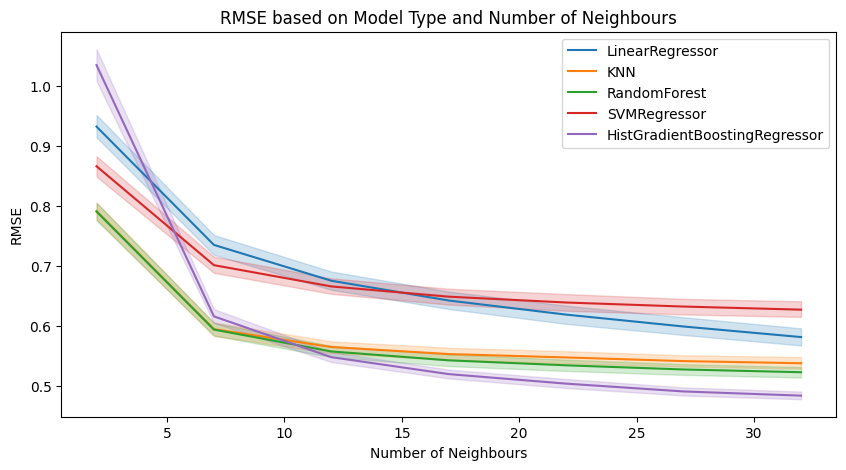
\includegraphics[width=1\textwidth]{images/rmse_by_model_type.png}
  \caption{RMSE by Model Type with the Confidence Interval of 95\%}
  \label{fig:rmse by model type}
\end{figure}

\subsection{Model Comparison}

First, we compare the overall performance of the models against each other. Figure~\ref{fig:rmse by model type} shows the RMSE of each model accross both Hamburg and Stuttgart for the month of June 2023. For all models, one evaluation was done using the imputed dataset without missing values, as Linear Regression, KNN, Random Forest and SVM Regression cannot handle missing values. Gradient Bootsting was once run with and once run without imputed data, where the imputed data performed better at 2 neighbours, possibly due to neighbours with missing values, but performed slightly worse than not imputed data for higher amounts of neighbours. SVM, KNN and Random Forest seem to hit a plato when reaching a certain number of neighbours, around 15-20, whereas Linear Regression and Gradient Boosting continue to improve with a higher number of neighbours.\\
Gradient Boosting shows the lowest RMSE starting with over 10 neighbours and has the smallest confidence interval. The non imputed data also performs slightly better, as seen in Appendix (TODO: Link), therefore we will continue a more detailed evaluation with the Gradient Boosting model without imputed data. It is to note, that the individual models were mainly run with default parameters as given by sklearn library, therefore the performance of the individual models could be further improved. The exact parameter configurations can be found in Appendix~\ref{appendix: sklearn ml parameters single station}.

\subsection{Further Evaluation - Gradient Boosting}

HistGradientBoostingRegressor without imputation achieves overall the lowest RMSE starting with more than 10 neighbours and continously improves with more neighbours, however the improvements after 30 neighbours are really small. This model is great because it has native NaN support and we can save the imputation step that can possible introduce bias into the model. The difference to KNN and Random Forest is not that big with a little less than RSME of 0.1, however the confidence interval is also smaller compared to the other models. Due to the lowest error and performance benefits compared to other models such as Random Forests and no need to use imputation, the HistGradientBoostingRegressor is used in the following section to further investigate feature importance, the influence of different time intervals and the impact of QC on the process.\\

\begin{figure}[htp]
    \centering
    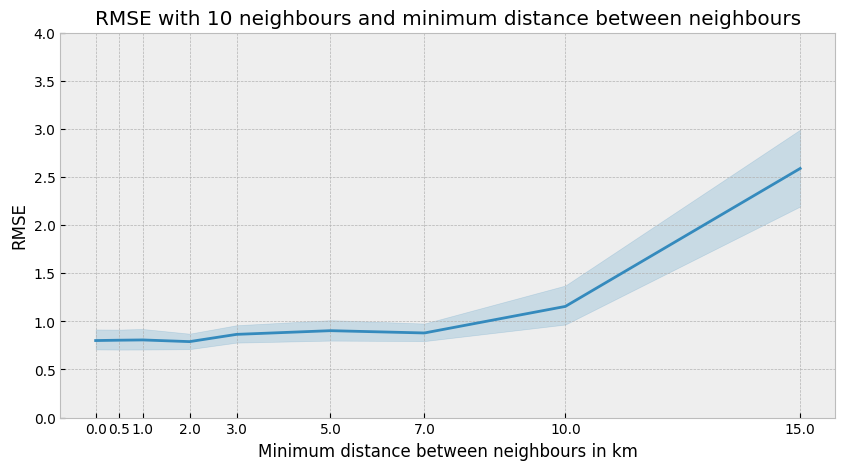
\includegraphics[width=1\textwidth]{images/rmse_10_neighbours_min_distance.png}
    \caption{RMSE for Increasing Minimum Distance with 10 Neighbours, Hamburg, Netatmo}
    \label{fig:eval hamburg minimum distance between stations}

    \centering
    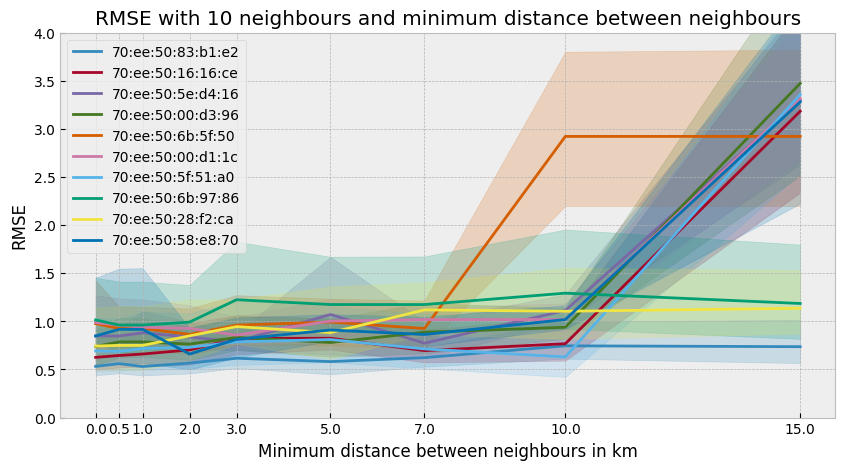
\includegraphics[width=1\textwidth]{images/rmse_10_neighbours_min_distance_by_pid.png}
    \caption{RMSE for Increasing Minimum Distance with 10 Neighbours By Station Id, Hamburg, Netatmo}
    \label{fig:eval hamburg minimum distance between stations by station id}
\end{figure}

\subsubsection{Influence of Distance between Neighbours}

% Hypotheses: closer neighbours have a higher influence on the temperature
The goal with hyperlocal temperature mapping is to get a deep insight into very local climatic conditions. If two sensors are located in the same climatic conditions, in an extreme case directly situated next to each other, both sensors should measure the same temperature. Therefore the hypotheses is, that closer stations have a higher influence on the prediction quality, e.g.\ if closer stations are choosen as neighbours the prediction quality is better compared than if the same number of neighbours is choosen but further away. We investigate this hypotheses by comparing the RMSE of prediction quality for different distances between neighbours. Because there are not so many stations available for Hamburg, that for example 10 stations could be selected in a 500m radius, we look at the minimum distance instead and remove neighbours that are to close to the station.\\
The evaluation is done using 5-fold cross validation for a subset of 10 stations in Hamburg, spread across a bigger area so we can cover different distances between neighbours and different climatic conditions, e.g.\ distance to water, situated in the city centre etc. The list of stations can be found in Appendix~\ref{appendix stations for minimum distance between stations}. The number of neighbours was set to 10 as this number was the number at which Gradient Boosting putperformed other models. Figure~\ref{fig:eval hamburg minimum distance between stations} shows the RMSE for different minimum distances between stations in km for 10 stations from Netatmo in Hamburg with 10 neighbours. We can see that the RMSE is increasing minimally across the first few kilometres and then starts to sharply increase with greater distances over 10km. However, if we take a look at Figure~\ref{fig:eval hamburg minimum distance between stations by station id} which shows the same data but grouped by station id, we can see that there are several stations whose RMSE does not increase with greater distances.\\ % Todo: why?

\subsubsection{Feature Importance}

Next to the temperature, there are also other features that could be included in the prediction process such as the time, humidity, pressure, etc. In order to understand how much the features contribute to the overall prediction quality, we first compare the RMSE of the model with only the temperature as input feature for each neighbour, and then test with adding time, humidity, pressure, and finally all features combined. Time is only a single column of the transformed timestamp, whereas humidity and pressure are added for each neighbour. In the end the input looks as follows: [ta\_1... ta\_n, time, humidity\_1... humidity\_n, pressure\_1... pressure\_n]\\
Figure~\ref{fig:eval feature importance 10 stations single location} shows the RMSE for different features for 10 stations in Hamburg with 30 neighbours. We can clearly see, that there is no visible difference between only temperature and all features combined, therefore in Figure~\ref{fig:eval permutation importance single station} we take a look at the permutation importance of a single station for temperature and time on a 30\% test set. The values are calculated based on the trained regressors from the 5 different folds of the cross validation, however the test set was always the same and not the same used during the cross-validation, due to technical limitations in the sklearn library. However, the results indicates that only a very small number of stations, in this case the neighbours 4 and 13, have a high influence on the prediction quality. All other stations have a very low influence on the prediction quality, with time having no visible influence at all. This is a very interesting result, as it indicates that the model only needs a handful of neighbours that have similar temperature distributions to the target station in order to make a good prediction. Other features such as time, humidity and pressure do not seem to have any influence on the prediction quality, and could therefore be ignored, saving computational resources and making the model more robust. This assumption could be further validated by looking at more stations and their permutation importance.\\ 

\begin{figure}[htp]
    \centering
    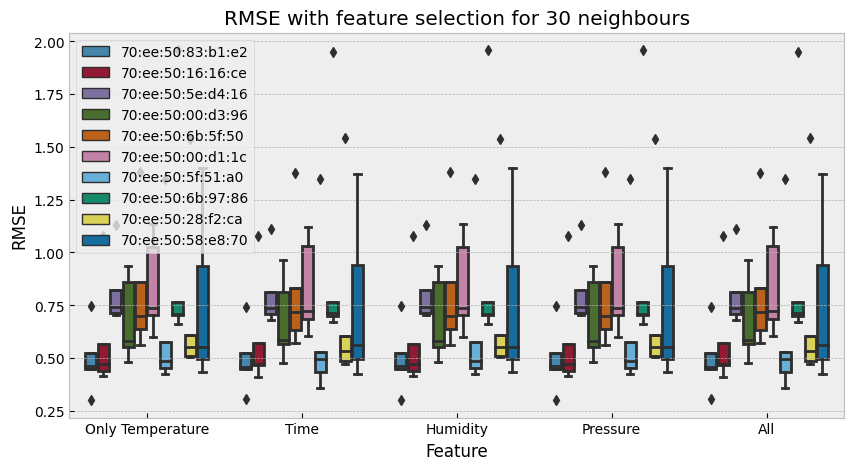
\includegraphics[width=1\textwidth]{images/rmse_30_neighbours_feature_importance_by_pid.png}
    \caption{RMSE based on Features Selected with 30 Neighbours, Hamburg, Netatmo}
    \label{fig:eval feature importance 10 stations single location}

    \centering
    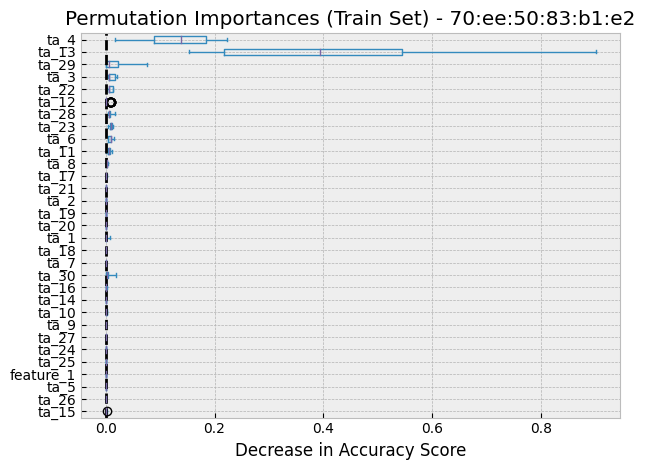
\includegraphics[width=1\textwidth]{images/rmse_30_neighbours_permutation_importance_by_pid.png}
    \caption{Permutation Importance for Single Station on 5-Fold Cross Validation, Hamburg, Netatmo}
    \label{fig:eval permutation importance single station}
\end{figure}

\subsubsection{Influence of Quality Control, Time Intervals and Non-Stationary Sensors}

% Inplicitly included via QC process, because many values are already missing -> check for subset with more data available how missing values influence the model
% - compare m4 vs m5

Sensor networks have the advantage, compared to remote sensing approaches, that they provide high temporal resolutions, however at the cost of spatial coverage. Related studies in the field of sensor networks suggest, %TODO: cite
that stationary sensor networks show less variability, but suffer from lower spatial coverage. In comparison, fully mobile sensor networks have a higher spatial coverage, but suffer from higher variability. Combining both approaches could therefore be a promising approach to increase the spatial coverage of the sensor network, while still maintaining a high prediction quality.\\
In the context of air temperature sensing, air temperature sensors could be mounted to busses, cars, scooters, or bikes. Unfortunately, there are currently no such datasets available, however we can simulate a non-stationary sensor by removing data points of specific sensors in either a fixed interval, e.g.\ simulating a bus line that visits a certain location in a rather fixed interval, or randomly, simulating a bike or scooter that is used periodically.\\
We have already indirectly simulated missing data by applying QC steps before using the station data to train the models, as seen in Section~\ref{sec:quality control}, where we lose quite some data, especially for Sensor.Community in the m5 buddy check. In order to further investigate the influence of missing data, we instead of using data that passed the m5 check, we will use data that passed the m4 check, which is less strict and therefore has more data available. An interesting exploration could be to use the previous sensor with Netatmo Station Id \textit{70ee:50:83:b1:e2} and choose on of the neighbours that has a high influence on the prediction quality, e.g.\ neighbour 4, and remove data points in both fixed and random intervals to simulate a moving sensor instead of a stationary sensor. We could also check what happens, if not only one but multiple neighbours are turned into simulated moving sensors, maybe with different intervals.\\
First, we need to get an understanding how the different QC steps influence the interpolation process. Therefore, we compare the RMSE for both m4 and m5 QC step for the 10 already used stations with 30 neighbours and the time feature.

% TODO: add figure for m4 vs m5
% TODO: add figure for different time intervals

% TODO: optional
% \subsubsection{January vs June}

% TODO: optional
% \subsubsection{Neural Network Exploration}

% Areal Interpolation
\section{Areal Interpolation of Air Temperature}

The second use-case for ML-based interpolation of air temperature is the areal interpolation, e.g.\ turning a set of single data points into a continuous temperature grid. The problem with this approach is that in comparison to interpolating a single sensor, there are potentially many locations that have no sensor data and therefore no target variable to be trained with. The main assumption here is that locations with similar features, e.g.\ land coverage, soil temperature, sky view factor, solar radiance, etc.\ have similar air temperature. The main challenge here is to find the right features that capture the dependency between the different locations.\\
In the first step, we simply use the coordinates of each data point in order to train the model in addition to remote sensing data, as land coverage and surface roughness have a high impact on air temperature.(Cite LCZ studies).
Further improvements

- parameters:
  - grid cell size

- todos:
  - try to get surface temperature for specific time step -> LST high influence on TA?

\subsection{Model Comparison}

- more features compared to location interpolation: land coverage, soil temperature, sky view factor, from satellite data and google earth engine

- improvements:
  - predict air temperature based on LST for better training

baseline: mean, IWD, ordinary kriging (with different kernels)

\subsection{Geostatistical Interpolation Baseline}
In order to evaluate the performance of the ML model, we need to first get a better understanding of the interpolation quality of existing interpolation techniques. Next to simpler deterministic interpolation methods, such as inverse weight distance (IWD) or k-nearest neighbours (KNN) that are easy and performant, but struggle to capture more complex interdependencies, there are also more complex methods available. The most common geostatistical method for interpolation is Krigin, which is based on a gaussian process and 

In the scope of this work, we unfortunately cannot compare all of these methods with each other and therefore need to focus on a subset of methods. EBK and EBKRP are one of the most commonly used methods for temperature interpolation (cite). According to \cite{njoku2023effects}, EBKRP continously outperforms EBK in different weather station density scenarios, therefore we will use EBKRP as a baseline for our comparison.\\
In the following, the machine learning fundamentals for this work are explained and the different ML regression model types are introduced.


\subsection{Further Evaluation - HistGradientBoostingRegressor}

\subsection{Datasets for Evaluation}

As a first step for training and testing areal air temperature interpolation methods, we need to define the test area and the data we use for training. In this context, it could be interesting to compare different sensor network providers.
For this use-case we have several test areas that we could validate. To get an overview of the sensors left after QC for Sensor.Community, Table 

-> could also compare with Hamburg (closer to water, more wind)

- find locations that are:
  - somewhat near reference stations for comparison
  - high station density
  - interesting features (e.g. parks, water, ...)

- locations in Germany for Sensor.Community are:
  - Stuttgart (birthplace of Sensor.Community) with high station density + one reference station somewhat close
  - Hamburg with lower sensor density, but 2 reference stations (interesting to see changes between those over realtively short distances) and close to water/river (Elbe)
  - other candidates (but with way fewer sensor and no reference stations): Cologne, Munich, Freiburg (interesting that they have an airport but no reference station), Lüneburg
  - interesting to note, that Berlin did not have any sensor stations that passed the QC step\\

\begin{figure}[ht]
    \centering
    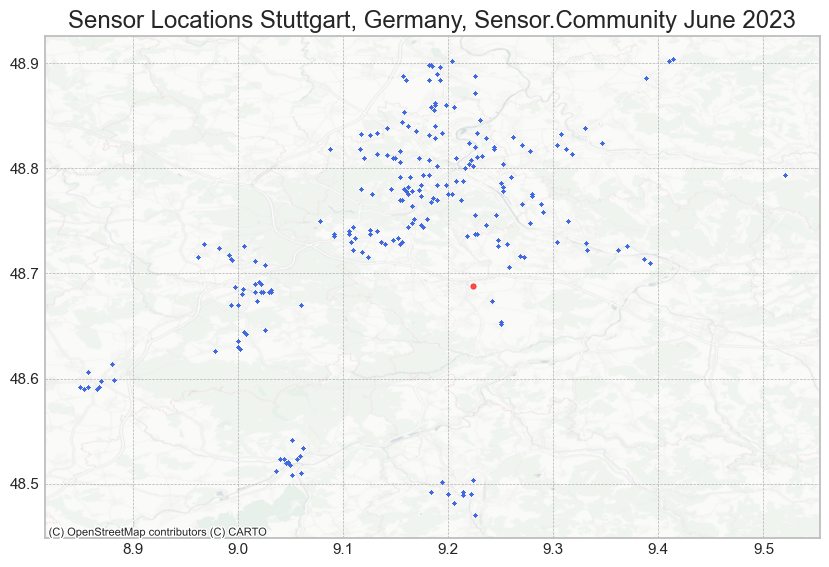
\includegraphics[width=1\textwidth]{images/sensor_community_locations_stuttgart_after_qc_june_23.png}
    \caption{Locations for Sensor.Community around Stuttgart, Germany, June 2023}
    \label{fig:qc sensor community stuttgart june 23}

    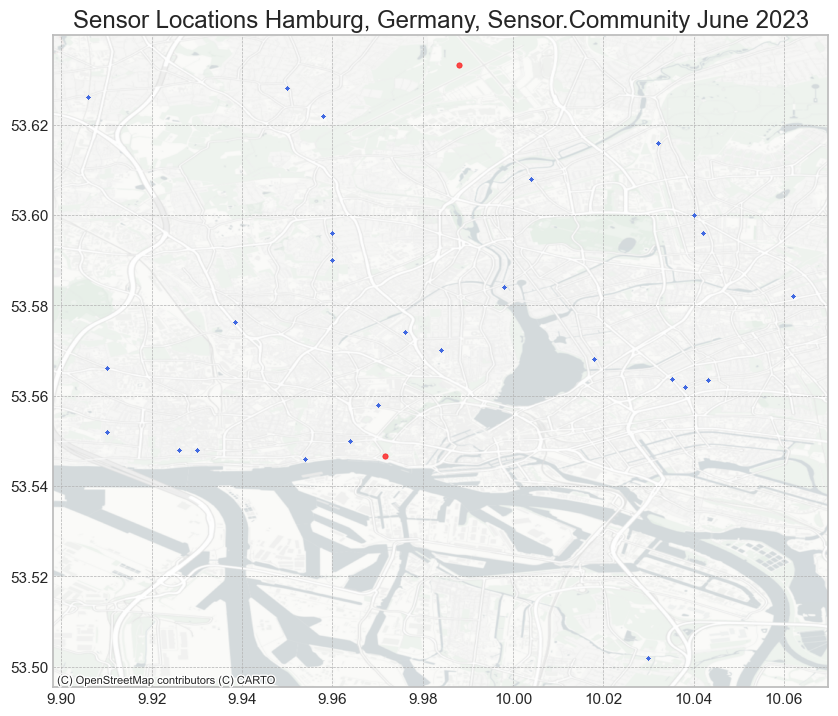
\includegraphics[width=1\textwidth]{images/sensor_community_locations_hamburg_after_qc_june_23.png}
    \caption{Locations for Sensor.Community in Hamburg, Germany, June 2023}
    \label{fig:qc sensor community hamburg june 23}
\end{figure}

- we choose stations from Stuttgart and Hamburg for the evaluation
-> identify stations with high mean daily temperature difference to reference station (to see if they are in a heat island)

\subsubsection{Stuttgart}

Station Locations:\\

\begin{figure}[ht]
    \centering
    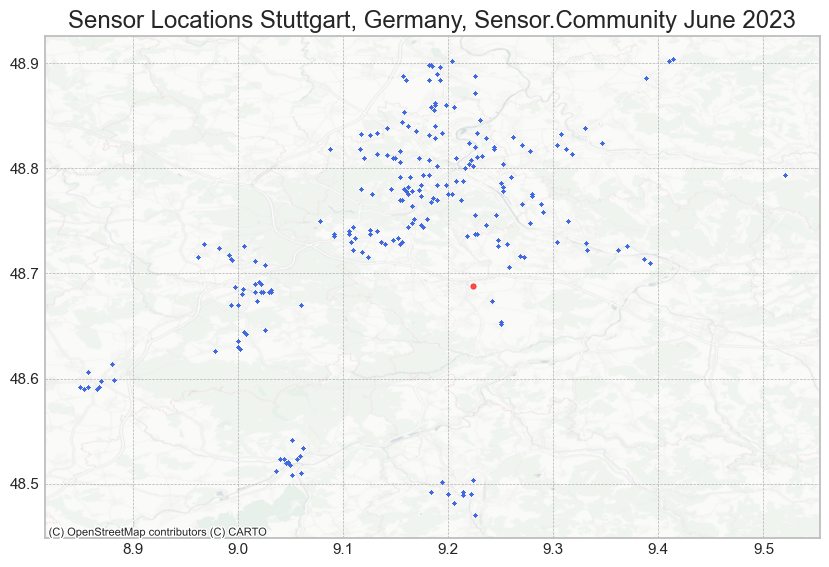
\includegraphics[width=1\textwidth]{images/sensor_community_locations_stuttgart_after_qc_june_23.png}
    \caption{Locations for Sensor.Community around Stuttgart, Germany, June 2023}
\end{figure}

DWD Reference location: 48.6883;9.2235 -> DWD id: 4931, Daily Max, Mean and Min values for June 2023\\

\begin{figure}[ht]
    \centering
    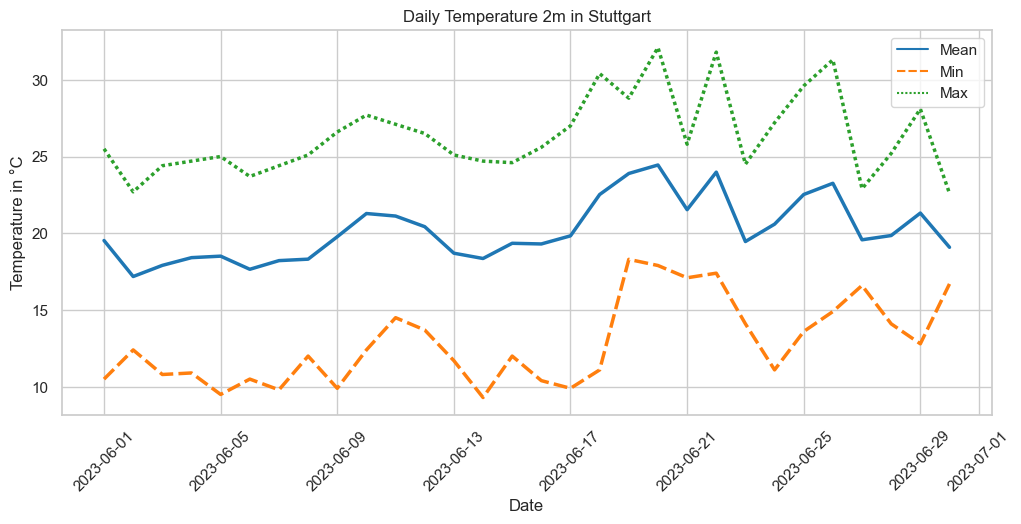
\includegraphics[width=1\textwidth]{images/dwd_stuttgart_june_23_tair_max_mean_min.png}
    \caption{Daily Mean, Max, and Min Air Temperature at 2m in Stuttgart, Germany, June 2023, DWD Station 4931}
    \label{fig:dwd mean max min stuttgart june 23}
\end{figure}

\subsubsection{Hamburg}

Todo: add Hamburg station locations\\

TODO
First compare only air temperature for stations that are near a reference station and have enough buddies for sensor community
- only for june 2023 from sensor community, not january as heat islands are not as important in winter (which depends on the context ofc if the goal is f.e. to save heating costs, could be a factor)

Steps in the evaluation:
- find sensor community stations near reference stations that passed m5 QC step
- Compare different interpolation approaches
  - linear, forests, KNN, NNetwork
  - with different amounts of data available (99\% -> 1\%) and see how RSME evolves


Steps:
- deterministic approaches
  - "naive" approach with nearest neighbor -> show high error rate
- probabilistic approaches
  - reference approach with geostatistical methods (ordinary kriging, empirical bayesian kriging, EBK with regression) -> still high error rate, especially with lower density of weather stations/bad support for irregularly spaced data
    - ordinary krigin:
        - temperature semivariogram first
        - add additional features (e.g. soil temperature, land coverage, sky view factor, ...) as semivariograms and use cokrigin to combine them
    - empirical bayesian kriging:
        - not implemented out of the box (pykrige)

  - semivariogram: https://pro.arcgis.com/en/pro-app/latest/help/analysis/geostatistical-analyst/understanding-a-semivariogram-the-range-sill-and-nugget.htm

- deep learning approach with neural networks -> itteratively improve model by adding additional features, compare with reference approach

% Overall steps

1. Data Collection and rough analysis
  1.1. Get data from Sensor.Community
  1.2. Get data from DWD
  1.3. Get data from satellites via Google Earth Engine
  1.4. Get data from Netatmo (Hamburg, try to get Stuttgart as reference with historical data via API)
2. QC steps (TA first)
  2.1. Try to remove indoor stations and stations with irregular data
  2.2. Remove stations based on buddy check (removes a lot of sensor community stations due to lower density)
  2.3. Reference station has high quality data already, but can be used as a reference (interesting the comparison from 2m TA to 5cm TA)
  2.4. Discuss QA for other parameters (Humidity, Pressure etc.)
3. Comparison of models
  3.1. Simple models with only coordinates as input features and TA as target feature
  3.2. Add additional features (land coverage (NDVI, EVI)) and see how they improve the model
    3.2.1. For land coverage etc.\ compare different satellites and resolutions
    3.2.2. For coordinates/distances, compare different ways of calculating distances or modelling them in the model
    3.2.3. Compare influence of normalization
  3.3. Try to create a more complex NN model to show capabilities of NNs and try out LSTM for time series
  3.4. Choose final candidate that seems the most promissing and compare with reference approach
4. Comparison with refrence approaches
  4.1. Compare with simple Ordinary Kriging approach (with different kernels)
  4.2. Discuss problem of not being able to extrapolate